
%%%%%%%%%%%%%%%%%%%%%%%%%%%%%%%%%%%%%%%%%%%%%%%%%%%%%%%%%%%%%%%%%%%%%%%%%%%%%%%%
%%%%%%%%%%%%%%%%%%%%%%%%%%%%%%%%%%%%%%%%%%%%%%%%%%%%%%%%%%%%%%%%%%%%%%%%%%%%%%%%
% DESIGN AND IMPLEMENTATION %
%%%%%%%%%%%%%%%%%%%%%%%%%%%%%%%%%%%%%%%%%%%%%%%%%%%%%%%%%%%%%%%%%%%%%%%%%%%%%%%%

\cleardoublepage
\chapter{Design and implementation}
\label{implementation}

In this chapter, all the phases of the project mentioned above are detailed. The evolution and description of each process and the problems encountered are described in each section.


\section{General architecture of Dr. Scratch} 
\label{sec:arquitectura}

Dr. Scratch is a client-server tool which analyzes the JSON file of a Scratch project. Its main architecture can be shown in the figure ~\ref{fig:architecture}. Clients make HTTP request to the server, which was allocated in a virtual machine of the Azure platform with Ubuntu 14.04.2 LTS as operative system. It was possible thanks to a free subscription of Microsoft. However, this subscription was over and the new version was migrated to the Google Cloud Platform, which will be detailed in the section \ref{subsec:mig_to_google}. 

The version 2.4.10 of Apache Web Server was installed inside of the virtual machine of Azure, the same as the mod\_wsgi which connects Azure with Django. In order to collect the information, Dr. Scratch used the version 5.5.43 of the MySQL database. 

Hairball and Kurt modules were also installed in the virtual machine because they were necessary for the analysis of the Scratch projects. Kurt is a Python library for working with the Scratch project files. Hairball analyzes the JSON file of the Scratch projects and returns the total mastery and the total number of bad smells that the project has. Hairball analyzes the blocks of the projects through different plugins.

 \begin{figure}
    \centering
    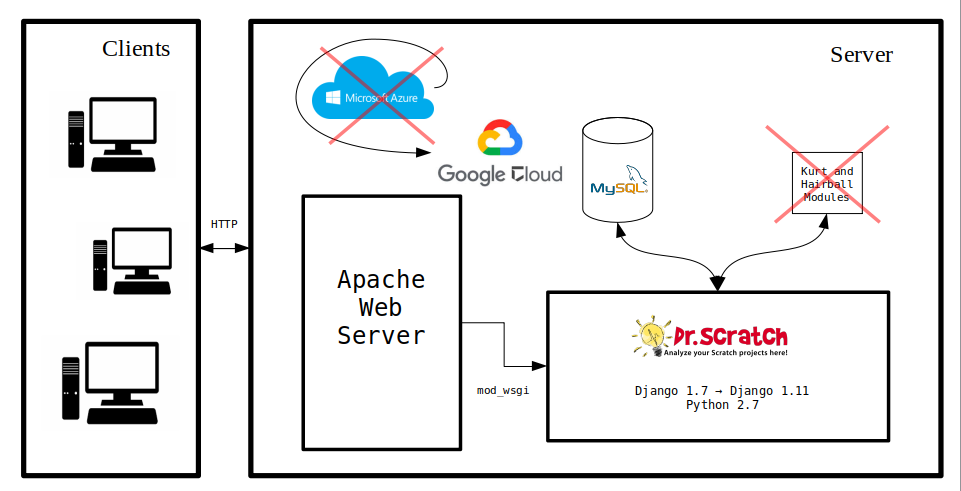
\includegraphics[width=11cm,                         keepaspectratio]{img/Client_Server.png}
    \caption{General architecture of Dr. Scratch.}
    \label{fig:architecture}
\end{figure}


\subsection{Dr. Scratch 3.0}
\label{subsec:newversion}

The starting point of this phase was the update of the Django version. The version 1.7 was obsolete, so we migrated the code to Django 1.11 LTS. 

On the other hand, the Scratch community announced the launch of the new version Scratch 3.0 in the coming months. From this point, we investigated their main changes. 

The most important modification was the structure of the JSON file of the Scratch projects. Hairball and Kurt modules were not compatible with the new format. Therefore, the first step was to modify these modules, since they only supported Scratch 1.4 an Scratch 2.0 versions. In order to simplify the tool, we decided to remove them instead to update them to the new version. In its place, we programmed some new scripts with the same functionality, but integrated into the main code. The objective was to develop different scripts which analyzed the total mastery of the CT development and the total number of bad smells in the Scratch project. 

Once that the functionality of Hairball module was replicated, we integrated the scripts in the main code of Dr. Scratch and removed the modules. We describe in more detail the scripts needed to replace the Hairball and Kurt modules below. 

\subsubsection{Mastery}
\label{subsubsec:mastery}

The \textit{analyzer.py} script analyzes the blocks of the JSON file and returns the punctuation of each of the seven categories of the CT which the Hairball module analyzed, the total mastery and the level of competence of the project. Each category is scored from 0 to 3 points, depending on the type of blocks. The total punctuation is the sum of the points of each category. Therefore, the range of the total mastery is from 0 to 21 points. Depending on the final mastery, the script differentiates three types of profiles (the same as Hairball module): basic (0-7 points), developing (8-15 points) or proficiency (16-21 points). In the Table ~\ref{table:competence_level} is detailed the evaluation of the competence levels~\cite{moreno2015dr}.

  \begin{table}
    \begin{center}
    \begin{tabular}{|c|p{4cm}|p{4cm}|p{4cm}|}
    \hline
     & \multicolumn{3}{|c|}{\textbf{Competence Level}} \\ \cline{2-4}
    \textbf{CT Concept} & Basic & Developing & Proficiency \\ 
    & (1 Point) & (2 Points) & (3 Points) \\ \hline  
    \textbf{Flow control} & Sequence of blocks. & Use of the repeat or forever blocks. & Use of the repeat until block. \\ \hline
    \textbf{Data representation} & Modifiers of sprites properties (looks, motion). & Operations on variables. & Operations on lists. \\ \hline
    \textbf{Abstraction} & More than one script or more than one sprite. & Definition of blocks. & Use of clones. \\ \hline
    \textbf{User interactivity} & Use of the green flag block. & Use of key pressed, sprite clicked, ask and wait or mouse blocks. & Use of video or audio sensing blocks. \\ \hline
    \textbf{Synchronization} & Use of the wait block. & Use of the broadcast and receive messages, stop all or stop program blocks. & Use of the wait until, when backdrop change to or broadcast and wait blocks. \\ \hline
    \textbf{Parallelism} & Two scripts on green flag. & On the same sprite, two scripts on key pressed or on sprite clicked. & Two scripts start with the same multimedia event, when broadcast received, when backdrop switches to or create clone. \\ \hline
    \textbf{Logic} & Use of the if block. & Use of the if else block. & Use of the operator blocks. \\ \hline
  \end{tabular}
  \caption{Competence Level for each CT concept.}
  \label{table:competence_level}
 \end{center}
\end{table}

\subsubsection{Sprite naming}
\label{subsubsec:sprite_naming}

 The \textit{spriteNaming.py} script analyzes the default names of the sprites (Sprite1, Sprite2, \ldots SpriteN) in the JSON file of the Scratch project. It returns the total number of default sprite names found and the list with all of them.

\subsubsection{Backdrop naming}
\label{subsubsec:backdrop_naming}

The \textit{backdropNaming.py} script analyzes the default names of the backdrops (Backdrop1, Backdrop2, \ldots BackdropN) in the JSON file of the Scratch project. It returns the total number of this bad smell and a list with the default names of the backdrops.

\subsubsection{Duplicated code}
\label{subsubsec:dup_code}

The \textit{duplicatedScripts.py} script analyzes the repeated block structures. It detects scripts, with more than five blocks, which are repeated in the same sprite or in a different one. It returns a dictionary in which the keys are the name of the sprites that have repeated code and the values are the duplicated scripts, respectively. In addition, it returns the total number of duplicated scripts found.

\subsubsection{Dead code}
\label{subsubsec:dead_code}

The \textit{deadCode.py} script analyzes unreachable code in isolated blocks or block structures in the analyzed Scratch project. The structures that it detects are:

\begin{itemize}
    \item Empty loop blocks: control blocks which do not have other blocks inside. 
    \item Empty conditions: control blocks which do not have conditions to execute the code inside of them.
    \item Hat blocks: structures which do not start with an event block (green flag, key pressed, etc.).
    \item No message: scripts which start with the `When broadcast received' block, but this message is never sent. 
    \item Dead code: blocks that do not have parent or next. Isolated blocks that are never executed.
\end{itemize}

Finally, this script returns a list of the dead code (scripts or isolated blocks) for each sprite and the total number of this bad smell.

\subsubsection{Attribute initialization}
\label{subsubsec:att_initialization}

The \textit{attributeInitialization.py} script tried to replace the Hairball plugin that checked if modified attributes were properly initialized. There are many blocks related to attributes in Scratch: costume, orientation, position, size and visibility. Due to the complexity of the code to analyze whether all of these properties were correctly initialized, it was so complicated to develop the same code in a script. Finally it did not work properly and the new script did not replace perfectly the plugin. For that reason, in the new version of Dr. Scratch this bad smell is not included.

\subsection{Migration of Dr. Scratch 3.0 to Azure Platform}
\label{subsec:mig_to_azure}

Before the launch of the new version of Dr. Scratch, we decided to test it during a period of time in another virtual machine of Azure. In the figure \ref{fig:migrations} we can observe the process from the development of the new version until its current deployment.

 \begin{figure}
    \centering
    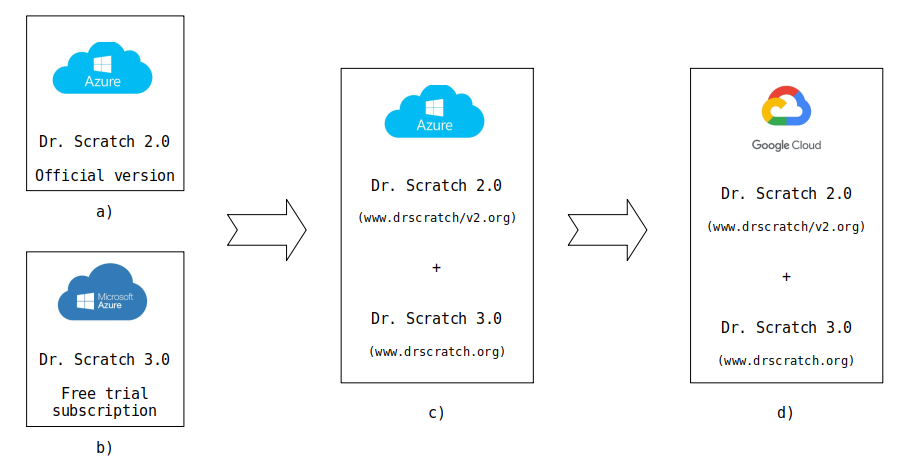
\includegraphics[width=11cm,                         keepaspectratio]{img/migrations.png}
    \caption{Migration process for the new version of Dr. Scratch.}
    \label{fig:migrations}
\end{figure}


Thanks to a educative subscription, we had a free trial period of the services offered by Azure during a month. In this way, we configured a virtual machine with the new version of Dr. Scratch and we tested it during a month, as we observe in the figure \ref{fig:migrations} b). To carry out this process, it was necessary to configure Apache throughout the file \textit{httpd.conf}. This file contained the main instructions. In addition, we needed a testing database with MySQL.

After correcting some small errors during the trial period, such as the download of certificates or the change of language,  we configured the official virtual machine of Azure with both versions of Dr. Scratch, as we observe in the figure \ref{fig:migrations} c). Again, it was possible thanks to the configuration of the file \textit{httpd.conf} of Apache. Finally, in January 2019 we launched the new version. Dr. Scratch 3.0 was allocated in the \textit{www.drscratch.org} domain. Its main page contained a link which redirected to the old version, allocated in the \textit{www.drscratch.org/v2} domain. We can observe the main interface of the tool in the figure ~\ref{fig:dr_scratch}.


\subsection{Migration of Dr. Scratch 3.0 to Google Cloud Platform}
\label{subsec:mig_to_google}

In April 2019, the funding which we received from Microsoft was over and we studied different options to allocate Dr. Scratch. Finally, the best solution was to migrate the application to the Google Cloud technology, as we can observe in the figure \ref{fig:migrations} d).
 
We received a grant from the GCP Research and, thanks to that, we configured the new services. We deployed a new virtual machine with 18.04.4 Linux as operative system. In addition, we updated MySQL to the 5.7.28 version. We migrated both versions to the new platform and we configured again the Apache module. It was a quick process and we had a short trial period. After solving small problems, we got a stable version which is working at present.


\section{Analysis of bad smells}
\label{sec:analysis}

Despite the new version Dr. Scratch 3.0 was stable in the new platform, all the analysis of bad smells was carried out with Dr. Scratch 2.0. The reason was that the data set used in the analysis were composed of projects with the old version of Scratch, that is, with the extension \textit{.sb2}.

Therefore, both data sets were analyzed with the Hairball module of Dr. Scratch 2.0. The Dr. Scratch tool in the previous version identified four different types of bad smells that can be present in Scratch projects: copy and pasted code (duplicate scripts) ~\cite{robles2017software}, the use of default names for sprites (default names), code that is never being executed (dead code), and variables that are not correctly initialized (attribute initialization). Their characteristics and impact are summarized in Table ~\ref{table:bad_smells}.

\begin{table}
 \begin{center}
  \begin{tabular}{ |p{4cm}|p{5cm}|p{5cm}|}
    \hline
    Bad Smell Type & Definition & Impact on Learning \\ \hline
    Duplicate scripts & Code is copy and pasted, sometimes with minor changes & It hinders the use of user-defined blocks and as such can be seen a limitation to the development of the abstraction skill \\ \hline
    Default names & Objects are not given a meaningful name, but keep the default {\em SpriteN} name & It hinders interaction among objects, as using them in other objects becomes more difficult \\ \hline
    Dead code & Code that is never being executed (usually because they do not have a starting condition) & It may indicate missing functionality \\ \hline
    Attribute initialization & Variables are not well initialized & It hinders the start of some objects, because their position, size, costume, etc are not correctly initialized \\ \hline
  \end{tabular}
  \caption{Type of bad smells.}
  \label{table:bad_smells}
 \end{center}
\end{table}

\subsection{Data set description}
\label{subsec:descrip_dataset}

In order to analyze the presence of bad smells, as well as their relationship with the level that users have in CT development, a large set of projects is necessary. In this work we have analyzed two different data sets. The first of them, which we will call data set a, was analyzed in a preliminary analysis. In order to improve and verify the results obtained, we repeat the analysis with a bigger data set, which we will call data set b. The description of both data sets is summarized in Table ~\ref{table:dataset}.

\begin{table}
 \begin{center}
  \begin{tabular}{|c|c|c|}
    \hline
    & \textbf{Number of projects} & \textbf{Number of snapshots} \\ \hline
    \textbf{Data set a} & 771 & 62,074 \\ \hline
    \textbf{Data set b} & 250,163 & - \\ \hline
  \end{tabular}
  \caption{Description of the data set used in the analysis.}
  \label{table:dataset}
 \end{center}
\end{table}


\subsubsection{Data set a}
\label{subsubsec:dataset_a}

The data set a was created and studied in another, previous research~\cite{troiano2019my}. A group of 438 students designed games for STEM using Scratch 2.0. During this process, the authors obtained snapshots of the process, in different periods of time, in order to show a temporary evolution. The total number of projects without taking into account the replicas over time, was 771. As a result, the complete data set was comprised of 62,074 projects formed by the different snapshots~\footnote{https://drive.google.com/drive/u/0/folders/1tDI6nx2f6344xJAKeUeWBeTg0YzxE3bO}. The objective of storing snapshots was to analyze the same 771 projects in different points of time.

\subsubsection{Data set b}
\label{subsubsec:dataser_b}

The data set b was also created and analyzed in another previous research~\cite{aivaloglou2017dataset}. This data set contained 250,163 Scratch projects, from more than 100,000 different users of its community. These projects were scraped from the Scratch repository. The scraper and all project files are available~\footnote{https://github.com/TUDelftScratchLab/ScratchDataset}. All the data was stored in two CSV files, \textit{metadata.csv} and \textit{code.csv}. These files included, for each Scratch project, its metadata, the program data, and the programming mastery scoring results from the Dr. Scratch assessment.


\subsection{Data collection}
\label{subsec:datacollection}

From this point, we needed to create our own CSV files from the data sets described in the section~\ref{subsec:descrip_dataset}. The process of the data set construction for the analysis is detailed in this section.

\subsubsection{Data set a}
\label{subsubsec:datacollection_a}

In order to analyze the 62,074 snapshots with the Dr. Scratch tool, it was necessary to create a script. This script, \textit{projects\_analyzer.py}, was programmed in Python. It opens each folder with the Scratch project and analyzes its JSON file. As we mentioned previously, the analysis was carried out with the Hairball module and all its plugins. The script returns a CSV file, \textit{evolution\_time\_results.csv}, with the total mastery, the score of each category of the CT, the data of the bad smells and information of the blocks for each snapshot. During the analysis process of all the snapshots, 2,158 were erroneous for different reasons: the project was saved incorrectly, the code contained special characters, etc. The final set of projects analyzed was 59,916.

In addition, we programmed another script to analyze the last version of each project. That is, a script to analyze the 771 projects without the temporary evolution. It returns another CSV file, \textit{final\_projects\_results.csv}, with the same structure than \textit{evolution\_time\_results.csv}, but storing only the last snapshot of each project. 

The statistics of valid projects and snapshots for the analysis are summarized in Table~\ref{table:datacollection_a}.

\begin{table}
 \begin{center}
  \begin{tabular}{|c|c|c|c|c|}
    \hline
     & \textbf{Total samples} & \textbf{Valid samples} & \textbf{Wrong samples} & \textbf{Survival ratio} \\ \hline
    \textbf{Projects} & 771 & 754 & 17 & 97,80\% \\ \hline
    \textbf{Snapshots}& 62,074 & 59,916 & 2158 & 96,52\% \\ \hline
  \end{tabular}
  \caption{Description of the final data set a used in the analysis.}
  \label{table:datacollection_a}
 \end{center}
\end{table}


\subsubsection{Data set b}
\label{subsubsec:datacollection_b}

The size of the data set b was much bigger than the data set a. For this reason, we found complications when we tried to open the file \textit{code.csv} and analyze it. Its analysis with a Python script was too slow and required too much storage space. Finally, the solution was to create a jupyter notebook and read and analyze the file line by line. In this way, we could join and select the useful information from the \textit{code.csv} and \textit{metadata.csv} files. The result of the jupyter notebook was a new CSV file, \textit{final\_dataset.csv}, composed of data from both files and with the structure which we wanted for the analysis: total mastery, the score of each category of CT and information about bad smells and the blocks. 

During the analysis process, we found wrong projects again. We found null data in the \textit{metadata.csv} file and special characters in the \textit{code.csv}. Finally, the number of valid projects was 231,024. The statistics of the valid samples for the data set b are summarized in Table~\ref{table:datacollection_b}.

\begin{table}
 \begin{center}
  \begin{tabular}{|c|c|c|c|c|}
    \hline
     & \textbf{Total samples} & \textbf{Valid samples} & \textbf{Wrong samples} & \textbf{Survival ratio} \\ \hline
    \textbf{Projects} & 250,163 & 231,024 & 19,139 & 92,35\% \\ \hline
  \end{tabular}
  \caption{Description of the final data set b used in the analysis.}
  \label{table:datacollection_b}
 \end{center}
\end{table}
    

\subsection{General analysis}
\label{subsec:generalanalysis}

The main objective of this phase was to analyze the presence of several bad smells in Scratch projects and how they relate to the development of CT skills. We carried out a preliminary analysis with the data set a in order to analyze to what extent bad smells are present in Scratch projects and what is its impact. Then, we repeated the same analysis with data set b in order to verify the results with a bigger set of projects. We developed both analysis with jupyter notebooks based on the CSV files generated in the previous section. 

The starting point of the general analysis was to raise the main research questions that we wanted to analyze. All the proposal, as well as the development of the analysis and the results obtained were published in the paper ``Bad Smells in Scratch Projects: A Preliminary Analysis''~\cite{vargas2019bad}. We developed this paper for the EC-TEL congress~\footnote{http://www.ec-tel.eu/} and we presented it in the TACKLE workshop~\footnote{https://sites.google.com/site/2019tackleworkshop/home} (the 2nd Systems of Assessments for Computational Thinking Learning) in Delft, Netherlands.

\subsubsection{RQ1. To what extent are bad habits present in Scratch projects?}
\label{subsubsec:RQ1}

In particular, we answer this question by offering the percentage of projects that have at least one type of bad smell. This question allows to see how frequent projects show a bad smell, hinting to the relevance of the topic. We expect a significant number of projects to contain bad smells.

\subsubsection{RQ2. Does the development of CT skills relate to the presence of bad smells?}
\label{subsubsec:RQ2}

We would like to find out if the presence of bad smells correlates with the complexity of the projects. Our hypothesis is that projects that have higher degrees of CT development will have less bad smells, as these may hinder the development of CT skills.

\subsubsection{RQ3. Do projects with more blocks have a higher number of bad smells?}
\label{subsubsec:RQ3}

More complex projects usually have more blocks. Thus having a single bad smell in a small, simple project may have less impact than in a project with hundreds of blocks. In the former case, the impact could be big, while in the latter it could be seen as an exception, with little impact.

To answer this question, for projects of the same level of CT development we calculate the ratio of the number of bad smells detected to the total number of blocks. We expect that this ratio decreases with an increase in the development of CT skills required to create the Scratch projects.

\subsubsection{RQ4. Can we find a relation among specific bad smells?}
\label{subsubsec:RQ4}

As by now, we have considered all type of bad smells together. In this question, we dig into each of them separately. It may be possible that some bad smells appear more frequently in projects of lower complexity, while others appear in more complex projects.

\subsubsection{RQ5. To which extent can bad smells be identified in each of the CT development phases?}
\label{subsubsec:RQ5}

Related to the previous question, we analyze how the different bad smell types appear in projects in the different stages of CT development. Therefore, we consider projects with a low complexity (basic), medium complexity (developing) and major complexity (proficiency) and compute how often they contain a specific type of bad smell.

We expect that several types of bad smells appear in the early phases (basic), while others are more prominent in more complex projects (proficiency). We assume therefore that learners that achieve higher levels of complexity have overcome certain bad smells due to having developed certain CT skills, while other bad smells appear in those more complex projects.


\subsection{Statistical analysis}
\label{subsec:statisticalanalysis}

After the general analysis, we decided to extend the study with a statistical analysis. The main objectives of this analysis were: 

\begin{itemize}
    \item To analyze the behaviour and distribution of each type of bad smell through Dr. Scratch, during the timeline of the projects.
    \item To analyze the impact on the development of the computational thinking skills.
    \item To carry out the t-student statistical study in order to measure the effect that bad smells have throughout a period of time. 
\end{itemize}

Therefore, this second study was based on the data set a, since it was necessary a temporary evolution of the projects. The number of projects analyzed in an initial phase was 754, and the total number of snapshots was 59,916.

In order to analyze the impact of the analysis about our variable of interest (computational thinking), it was necessary to measure the effect of the number of bad smells in the projects.

The appropriate analytical procedure to do that was the test t student for independent samples, which compares the measures obtained in two different groups for a given variable. These two groups will be the following populations:

\begin{itemize}
    \item[--] D0: The first snapshot in which the project gets 7 points in the mastery, measured with Dr. Scratch for each project. 
    \item[--] D1: The last snapshot of each project in D0.
\end{itemize}

We call each population as D0 and D1, respectively. The data set for the analysis is 452 snapshots, divided in 226 for each population. This distribution is summarized in Table~\ref{table:statistical_analysis_distribution}. Based on these researching groups, we developed different situations in the statistical analysis.

\begin{table}
    \centering
    \begin{tabular}{|c|c|c|}
        \hline
        \textbf{Total samples} & \textbf{Samples in D0} & \textbf{Samples in D1} \\ \hline
        452 & 226 & 226 \\ \hline
    \end{tabular}
    \caption{Description of the final data set used in the statistical analysis}
    \label{table:statistical_analysis_distribution}
\end{table}

\subsubsection{RQ1. Statistical analysis for the total number of bad smells}
\label{subsubsec:RQ1_statistical}

The first analysis was carried out for the total number of bad smells, that is, the sum of each type of bad smell. We selected two populations in two different situations and developed the t student analysis for both of them.

\begin{itemize}
    \item[--] Case 1
    \begin{enumerate}[(i)]
        \item Population A: projects in D1 which had less than 5 bad smells in D0 (N=129).
        \item Population B: projects in D1 which had more than 20 bad smells in D0 (N=11).
    \end{enumerate}
    \item[--] Case 2
    \begin{enumerate}[(i)]
        \item Population A: projects in D1 which had less than 5 bad smells in D0 (N=129).
        \item Population B: projects in D1 which had more than 15 bad smells in D0 (N=22).
    \end{enumerate}
\end{itemize}


\subsubsection{RQ2. Statistical analysis for default naming}
\label{subsubsec:RQ2_statistical}

We repeated the test t student for independent samples for each bad smell, in order to avoid the noise introduced by the sum of all the bad smells. We selected four situations for the analysis of default naming.

\begin{itemize}
    \item[--] Case 1
    \begin{enumerate}[(i)]
        \item Population A: projects in D1 which had 0\% of default names over the total number of sprites in D0 (N=137).
        \item Population B: projects in D1 which had more than 30\% of default names over the total number of sprites  in D0 (N=64).
    \end{enumerate}
    \item[--] Case 2
    \begin{enumerate}[(i)]
        \item Population A: projects in D1 which had 0\% of default names over the total number of sprites in D0 (N=137).
        \item Population B: projects in D1 which had more than 50\% of default names over the total number of sprites  in D0 (N=30).
    \end{enumerate}
    \item[--] Case 3
    \begin{enumerate}[(i)]
        \item Population A: projects in D1 which had 0\% of default names over the total number of sprites in D0 (N=137).
        \item Population B: projects in D1 which had more than 70\% of default names over the total number of sprites  in D0 (N=24).
    \end{enumerate}
    \item[--] Case 4
    \begin{enumerate}[(i)]
        \item Population A: projects in D1 which had 0\% of default names over the total number of sprites in D0 (N=137).
        \item Population B: projects in D1 which had more than 100\% of default names over the total number of sprites in D0 (N=22).
    \end{enumerate}
\end{itemize}


\subsubsection{RQ3. Statistical analysis for duplicated code}
\label{subsubsec:RQ3_statistical}

The data set composed of projects with duplicated code was too small. For that reason, we only selected one case of study with the following populations. 

\begin{itemize}
    \item[--] Case 1
    \begin{enumerate}[(i)]
        \item Population A: projects in D1 which had not duplicated code in D0 (N=217).
        \item Population B: projects in D1 which had at least 1 duplicated code in D0 (N=9).
    \end{enumerate}
\end{itemize}

\subsubsection{RQ4. Statistical analysis for dead code}
\label{subsubsec:RQ4_statistical}

For the statistical analysis of the dead code, we selected three different cases of study.

\begin{itemize}
    \item[--] Case 1
    \begin{enumerate}[(i)]
        \item Population A: projects in D1 which had 0\% of dead code over the total blocks in D0 (N=116).
        \item Population B: projects in D1 which had more than 20\% of dead code over the total blocks in D0 (N=73).
    \end{enumerate}
    \item[--] Case 2
    \begin{enumerate}[(i)]
        \item Population A: projects in D1 which had 0\% of dead code over the total blocks in D0 (N=116).
        \item Population B: projects in D1 which had more than 30\% of dead code over the total blocks in D0 (N=55).
    \end{enumerate}
    \item[--] Case 3
    \begin{enumerate}[(i)]
        \item Population A: projects in D1 which had 0\% of dead code over the total blocks in D0 (N=116).
        \item Population B: projects in D1 which had more than 50\% of dead code over the total blocks in D0 (N=28).
    \end{enumerate}
\end{itemize}

\subsubsection{RQ5. Statistical analysis for attribute initialization}
\label{subsubsec:RQ5_statistical}

Finally, the last t student analysis was carried out for the attribute initialization. In this case, we selected two different situations for the study. 

\begin{itemize}
    \item[--] Case 1
    \begin{enumerate}[(i)]
        \item Population A: projects in D1 which had 0\% of attribute initialization over the total blocks in D0 (N=68).
        \item Population B: projects in D1 which had more than 20\% of attribute initialization in D0 (N=15).
    \end{enumerate}
    \item[--] Case 2
    \begin{enumerate}[(i)]
        \item Population A: projects in D1 which had 0\% of attribute initialization over the total blocks in D0 (N=68).
        \item Population B: projects in D1 which had more than 30\% of attribute initialization in D0 (N=6).
    \end{enumerate}
\end{itemize}


\section{Bad smells model}
\label{sec:badsmells}

Once we developed all the analysis, we discovered that the presence of bad smells in the Scratch projects was very significant, as well as its effect on the computational thinking developing. All the results will be detailed in the section~\ref{chap:results}. 

Therefore, it was necessary to develop a new environment in the Dr. Scratch tool, in order to show in the first place the results about bad smells. We will call this new environment as bad smells model. 

As we described in section~\ref{sec:reference}, the dashboard of bad smells in Dr. Scratch was very small. The main objective of this phase was to replace the dashboards, shown in figure ~\ref{fig:dashboards}, for the new model with more visual information about bad smells, shown in figure~\ref{fig:bad_smells}. The process of developing the new model was composed of different phases.

\subsection{\textit{Scratchblocks} library}
\label{subsec:scratchblocks}

The dashboard of bad smells showed the information with text format. In this way, it was more difficult to understand the presence of bad smells in the projects and, consequently, to correct them. Therefore, the first phase was to replace the dashboard with the text by visual blocks.

The \textit{scratchblocks} library~\footnote{https://github.com/scratchblocks/scratchblocks} makes pictures of Scratch blocks from text. We included this library in the code of Dr. Scratch and created a new template with four dashboards, for each bad smell. In addition, we programmed a new script, \textit{sb3\_blocks\_mapper.py}, to map the name of the blocks from the JSON file to the \textit{scratchblocks} library.

From this point, we found the problem that the scripts developed in the Phase 1 of the project returned the information about bad smells in a format which \textit{sb3\_blocks\_mapper.py} could not interpret. 

\subsection{Improvement of the scripts}
\label{subsec:improvement_scripts}

The scripts which we developed in the Phase 1 of the project were designed to show the information in a text list. For this reason, we had to change the format of all of them and to adapt the list of results of each bad smell. In addition, we added new functionalities, detailed below:

\begin{itemize}
    \item[--] Sprite naming: detection of default naming for more languages (Personatge, Figura, O actor, Personaia).
    \item[--] Backdrop naming: detection of default naming for more languages (Fons, Atzeko oihala).
    \item[--] Dead code: differentiation of dead code for each sprite, shown in the figure~\ref{fig:dead_code}.
    \item[--] Duplicated code: differentiation and identification of the sprites who have the duplicated blocks, shown in the figure~\ref{fig:dup_code}.
\end{itemize}

\begin{figure}
    \centering
    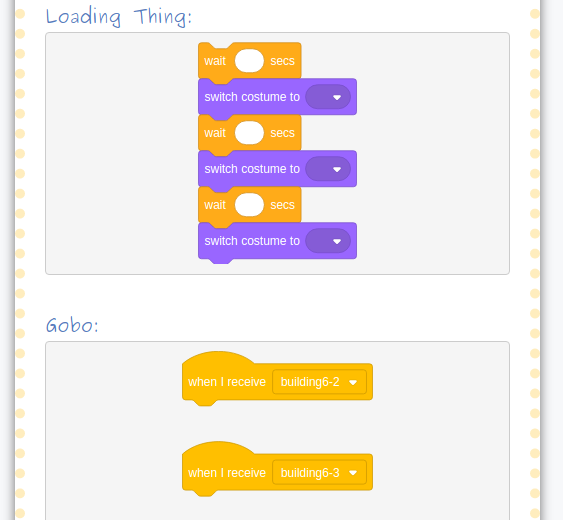
\includegraphics[width=9cm,                         keepaspectratio]{img/dead_code.png}
    \caption{Example of dead code for different sprites in the new bad smells mode.}
    \label{fig:dead_code}
\end{figure}

\begin{figure}
    \centering
    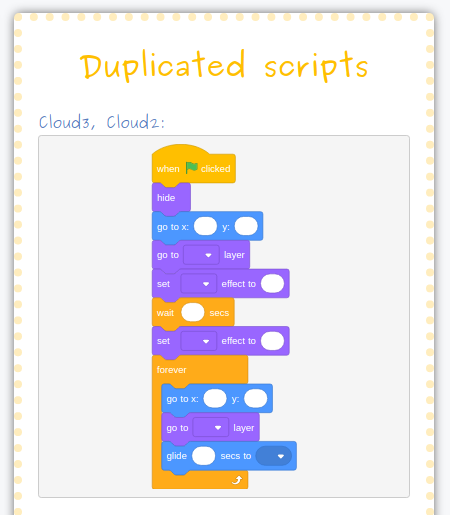
\includegraphics[width=9cm,                         keepaspectratio]{img/dup_code.png}
    \caption{Example of duplicated code for two sprites in the new bad smells mode.}
    \label{fig:dup_code}
\end{figure}


\subsection{Integration of the bad smells model in Dr. Scratch}
\label{subsec:integration_newmodel}

The last step for the development of the bad smells model was to integrate it in the Dr. Scratch code. When users analyzed a Scratch project with Dr. Scratch, they received the response with all the dashboards. We replaced this template for the template with the new model, which can be observed in the figure~\ref{fig:newmodel}.

\begin{figure}
    \centering
    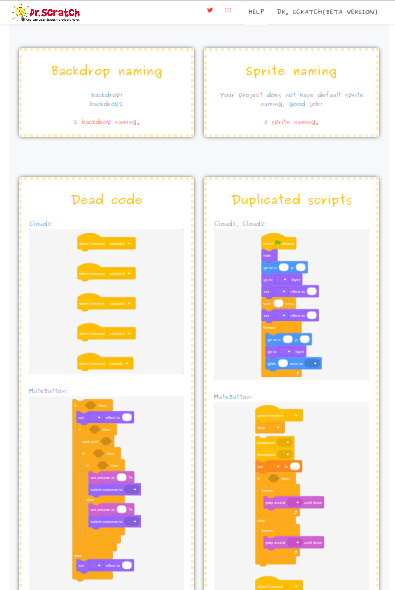
\includegraphics[width=12cm,                         keepaspectratio]{img/newmodel.png}
    \caption{Interface for the bad smells model.}
    \label{fig:newmodel}
\end{figure}

In addition, we added a new button to access the old dashboards. That is, once that users have analyzed their results related to bad smells, they can navigate to the rest of dashboards with the mastery results. We can observe this functionality in the figure~\ref{fig:button}.

\begin{figure}
    \centering
    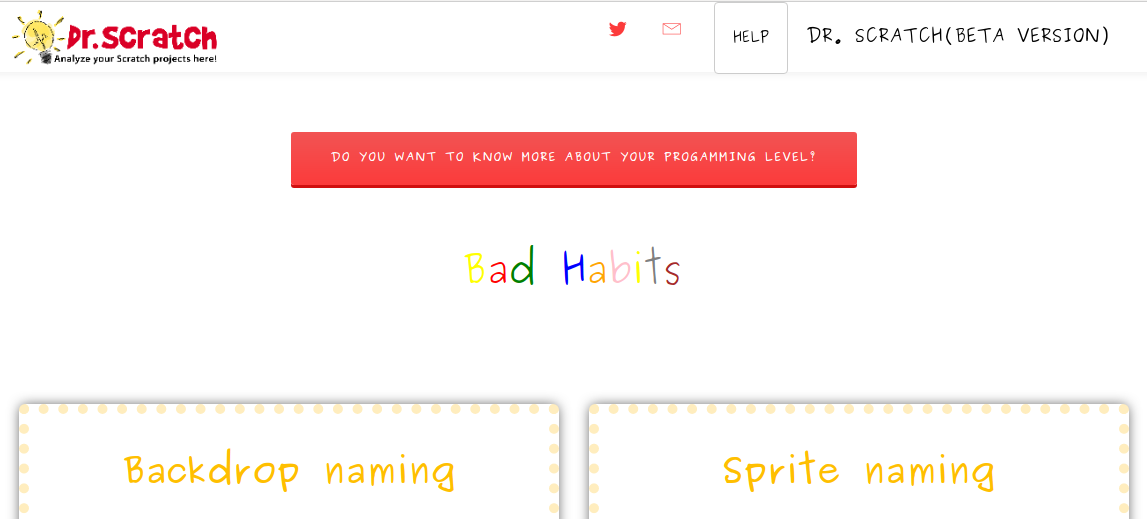
\includegraphics[width=8cm,                         keepaspectratio]{img/button.png}
    \caption{Button in the bad smells model to access the rest of the dashboards.}
    \label{fig:button}
\end{figure}

Finally, when the user profile was basic (from 0 to 7 points), the Dr. Scratch tool did not show the dashboard with the information about bad smells. Users who are beginning do not need so much information. For this reason, we though that it was better to avoid the bad smells model for this type of users. When the total mastery is less than seven points, Dr. Scratch shows the normal dashboards instead of the bad smells model, as we can observe in figure~\ref{fig:basic_level}.

\begin{figure}
    \centering
    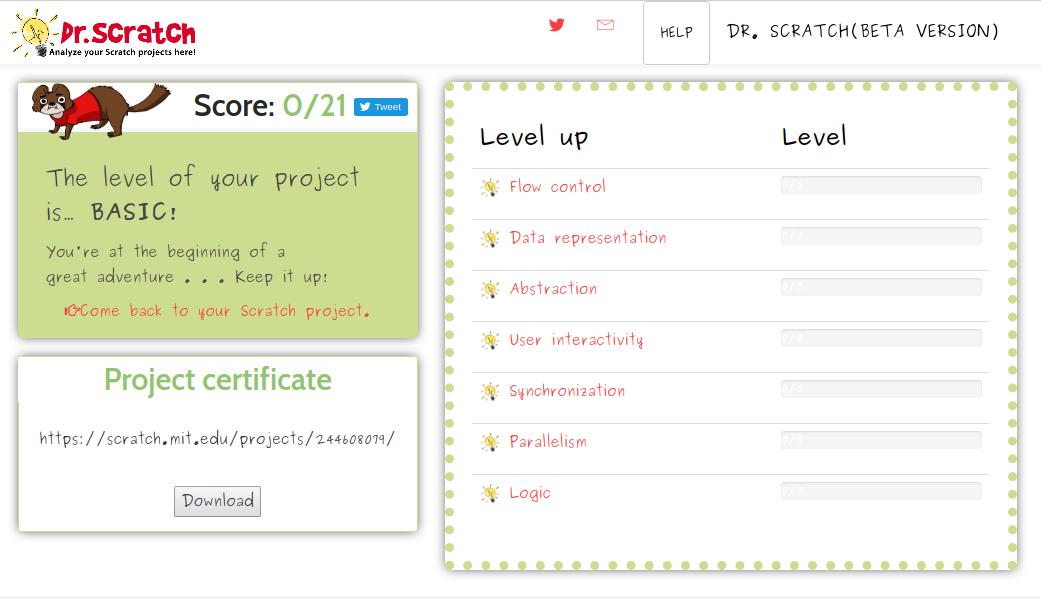
\includegraphics[width=8cm,                         keepaspectratio]{img/basic_level.png}
    \caption{Interface for users with basic profile.}
    \label{fig:basic_level}
\end{figure}


\section{Assessment experiment}
\label{sec:experiment}

\begin{itemize}
    \item Documento de ética: descripción general del experimento y contexto.
    \item Preparación del experimento y recursos necesarios.
    \item Recolección de datos del experimento.
    \item Desarrollo del experimento.
    \item Resultados generales del experimento.
\end{itemize}
